\documentclass{article}
\usepackage{listings}
\usepackage[T1]{fontenc}
\usepackage{titlesec}
\usepackage{graphicx}
\usepackage{amsmath}
\usepackage{xcolor}
\usepackage{amssymb}
\usepackage{circuitikz}
\usepackage{trace}
%\usepackage{minted}
\titleformat{\section}  % which section command to format
  {\fontsize{10}{12}\bfseries} % format for whole line
  {\thesection} % how to show number
  {1em} % space between number and text
  {} % formatting for just the text
  [] % formatting for after the text
  \title{Logika Cyfrowa}
\author{Jakub Gałaszewski} 
\begin{document}
\maketitle
\section{Poniższy kod implementuje rejestr przesuwny z liniowym sprzężeniem zwrotnym (linear-feedback shift register, LFSR). Jak wygląda jego sekwencja odliczania (zaczynając od 001)?}
\begin{center}
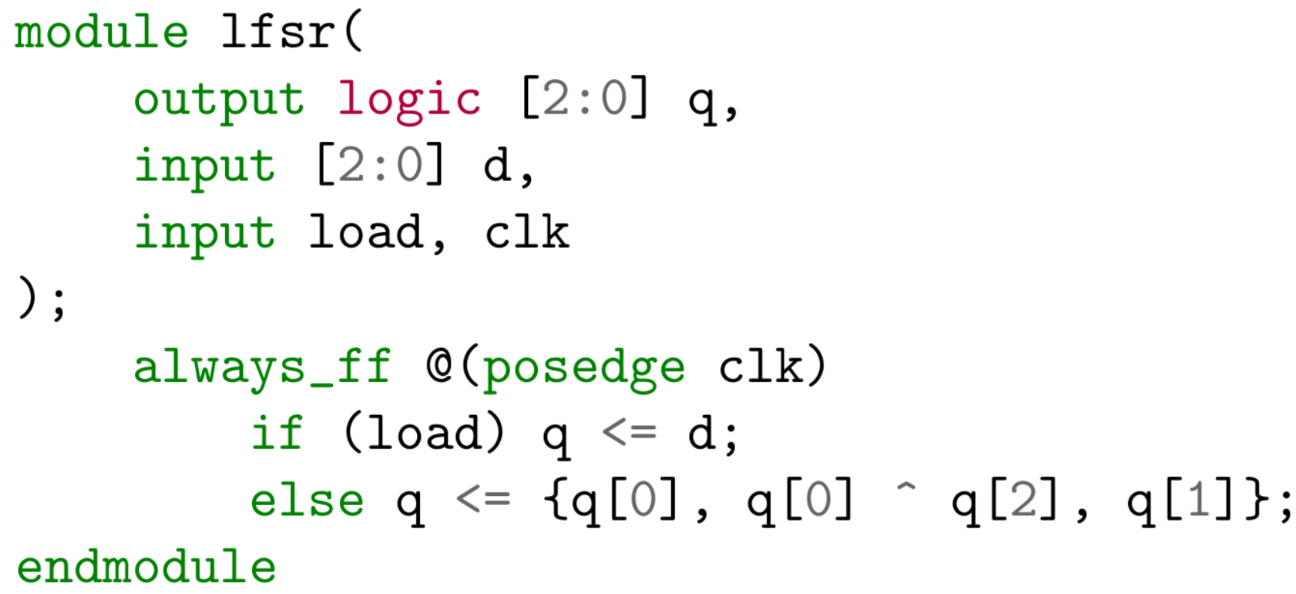
\includegraphics[scale=0.2]{./L08Z01.png}
\end{center}
\begin{center}
	$$q <= \{q[0], q[0] \oplus q[2], q[1]\};$$
	\begin{tabular}{|c|c|c||c|c|c|} 
	 \hline
	$q[0]$ & $q[1]$ & $q[2]$ & $q[0]'$ & $q[1]'$ & $q[2]'$ \\ 
	 \hline \hline
	 0&0&0&0&0&0\\ \hline
	 0&0&1& 1&1&0\\ \hline
	 1&1&0& 0&1&1\\ \hline
	 0&1&1& 1&1&1\\ \hline
	 1&1&1& 1&0&1\\ \hline	 
	 1&0&1& 1&0&0\\ \hline
	 1&0&0& 0&1&0\\ \hline
	 0&1&0& 0&0&1\\ \hline
	\end{tabular}
\end{center}
\section{Poniższy kod implementuje inny rejestr przesuwny z liniowym sprzężeniem zwrotnym. Jak wygląda jego sekwencja odliczania?}
\begin{center}
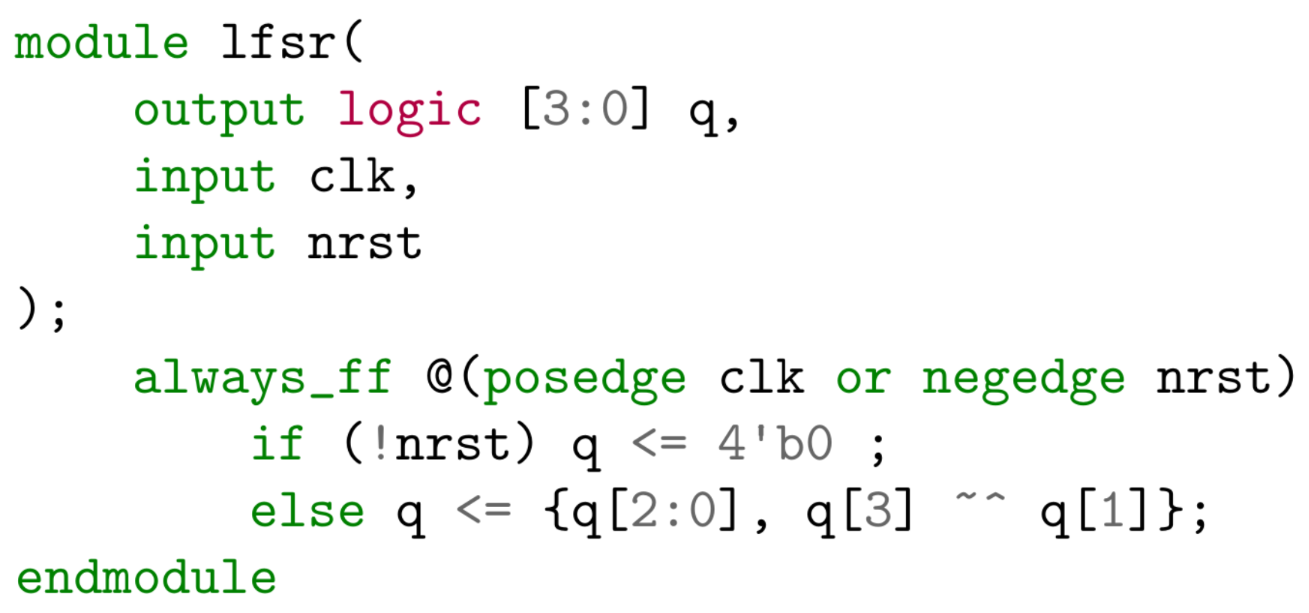
\includegraphics[scale=0.2]{./L08Z02.png}
\end{center}
\begin{center}
	$$q <= \{q[2:0], q[3] \neg \oplus q[1]\}$$
	\begin{tabular}{|c|c|c|c||c|c|c|c|} 
	 \hline
	$q[0]$ & $q[1]$ & $q[2]$ & $q[3]$ & $q[0]'$ & $q[1]'$ & $q[2]'$ & $q[3]'$ \\ 
	 \hline \hline
	 0&0&0&0& 0&0&0&1\\ \hline
	 0&0&0&1& 0&0&1&1\\ \hline
	 0&0&1&1& 0&1&1&0\\ \hline
	 0&1&1&0& 1&1&0&0\\ \hline
	 1&1&0&0& 1&0&0&0\\ \hline	 
	 1&0&0&0& 0&0&0&0\\ \hline \hline
	 
	 0&0&1&0& 0&1&0&0\\ \hline
	 0&1&0&0& 1&0&0&1\\ \hline
	 1&0&0&1& 0&0&1&0\\ \hline\hline
	 
	 0&1&0&1& 1&0&1&1\\ \hline
	 1&0&1&1& 0&1&1&1\\ \hline
	 0&1&1&1& 1&1&1&0\\ \hline
	 1&1&1&0& 1&1&0&1\\ \hline
	 1&1&0&1& 1&0&1&0\\ \hline
	 1&0&1&0& 0&1&0&1\\ \hline \hline
	 
	 1&1&1&1& 1&1&1&1\\ \hline \hline
	\end{tabular} 
\end{center}
\section{Rozważ poniższy blok always$_{ff}$:}
\begin{center}
	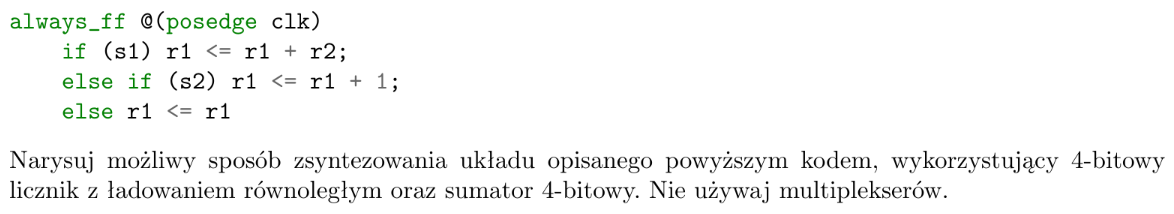
\includegraphics[scale=0.4]{./L08Z03.png}\\
	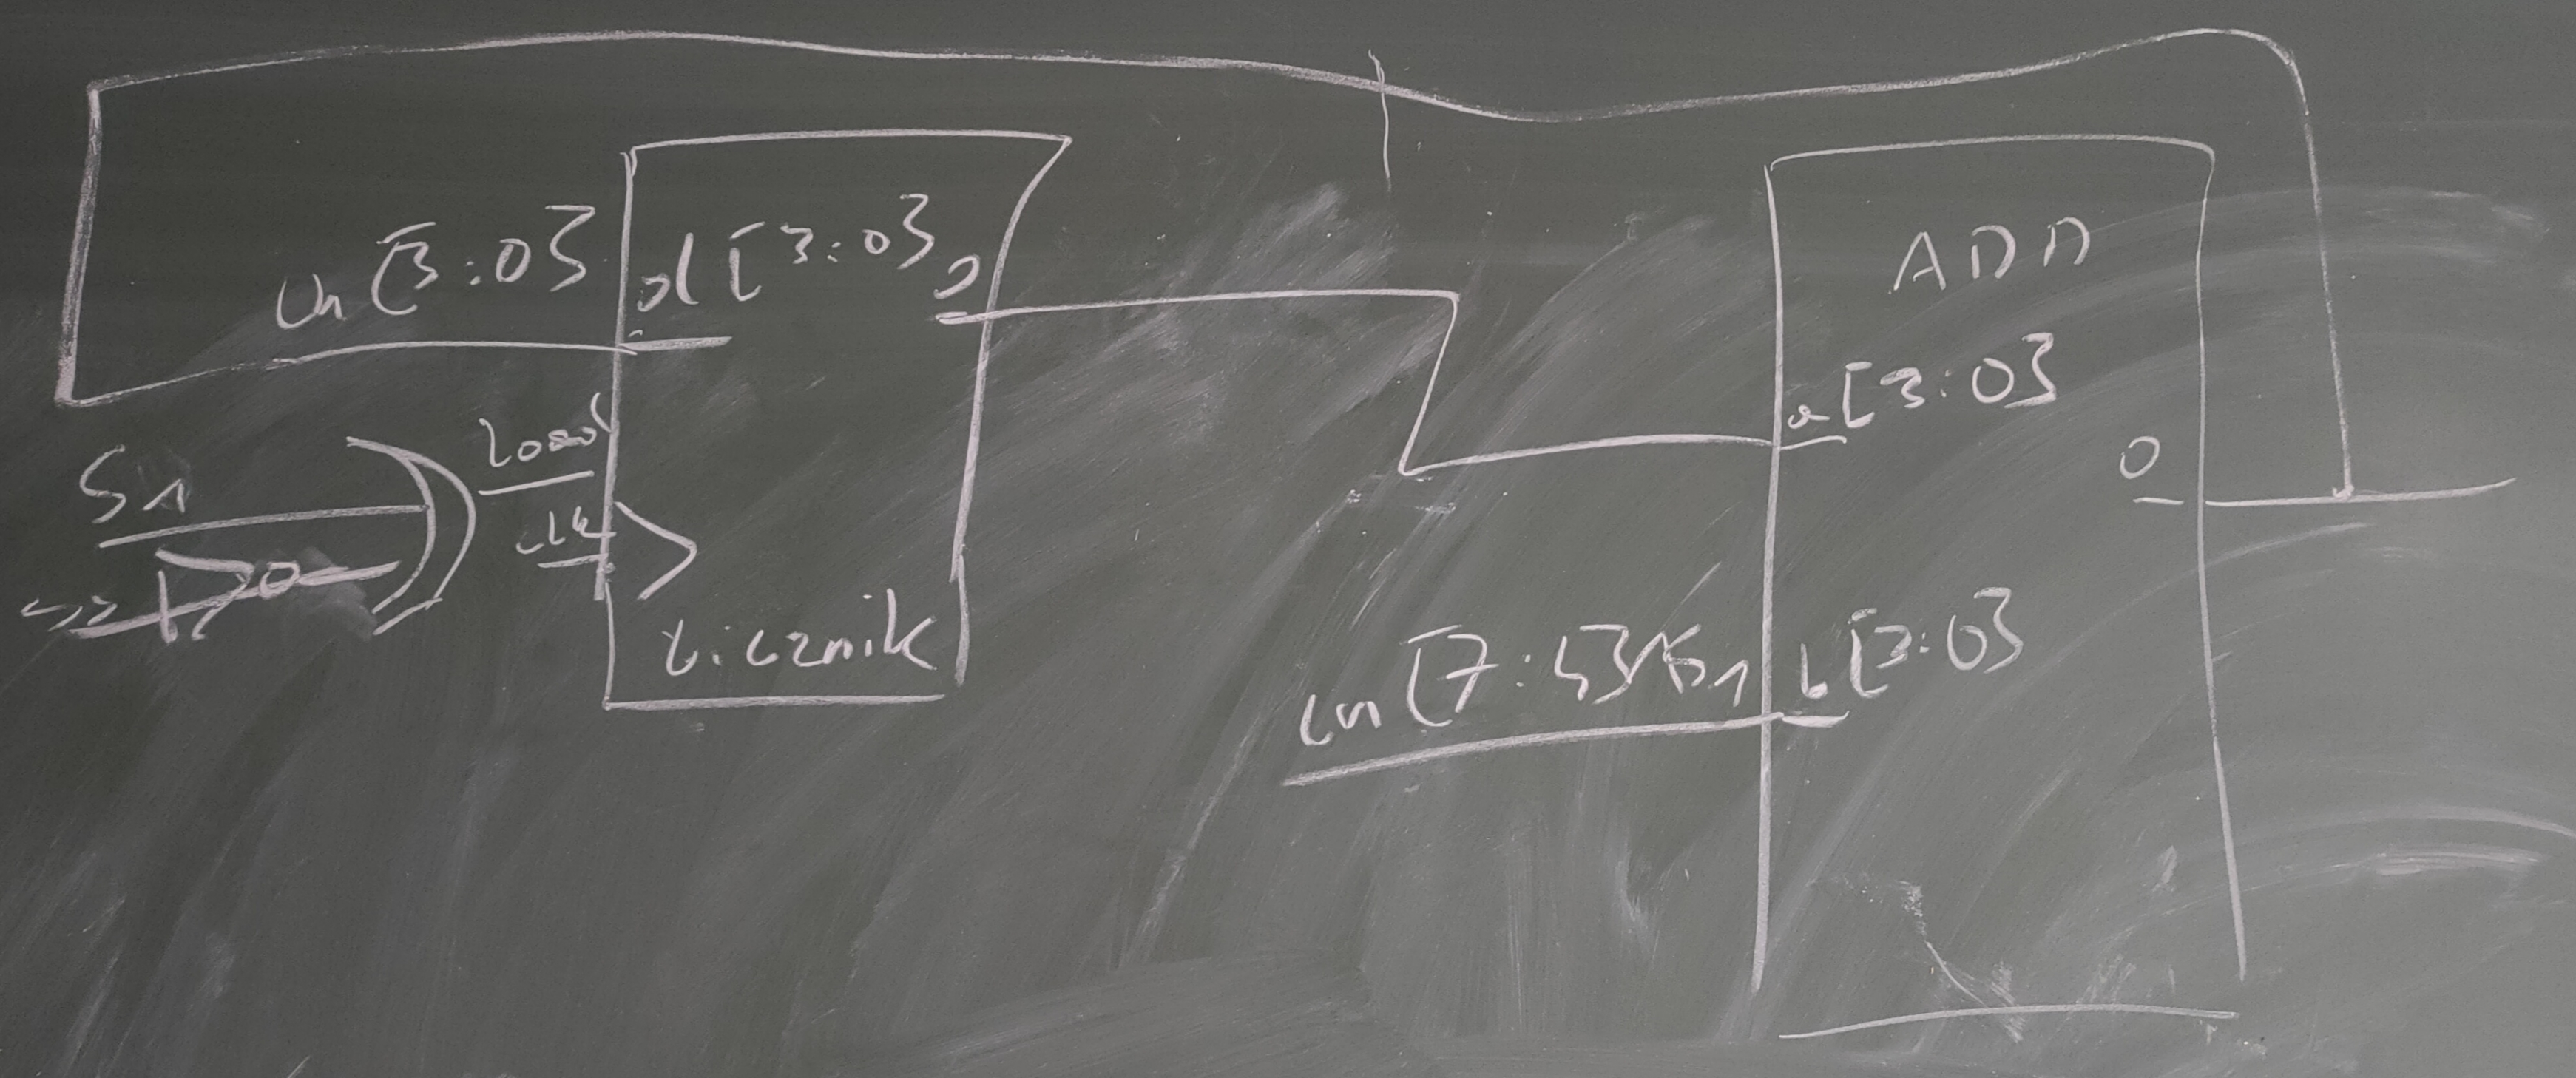
\includegraphics[scale=0.1]{./L08Z03.jpg}
	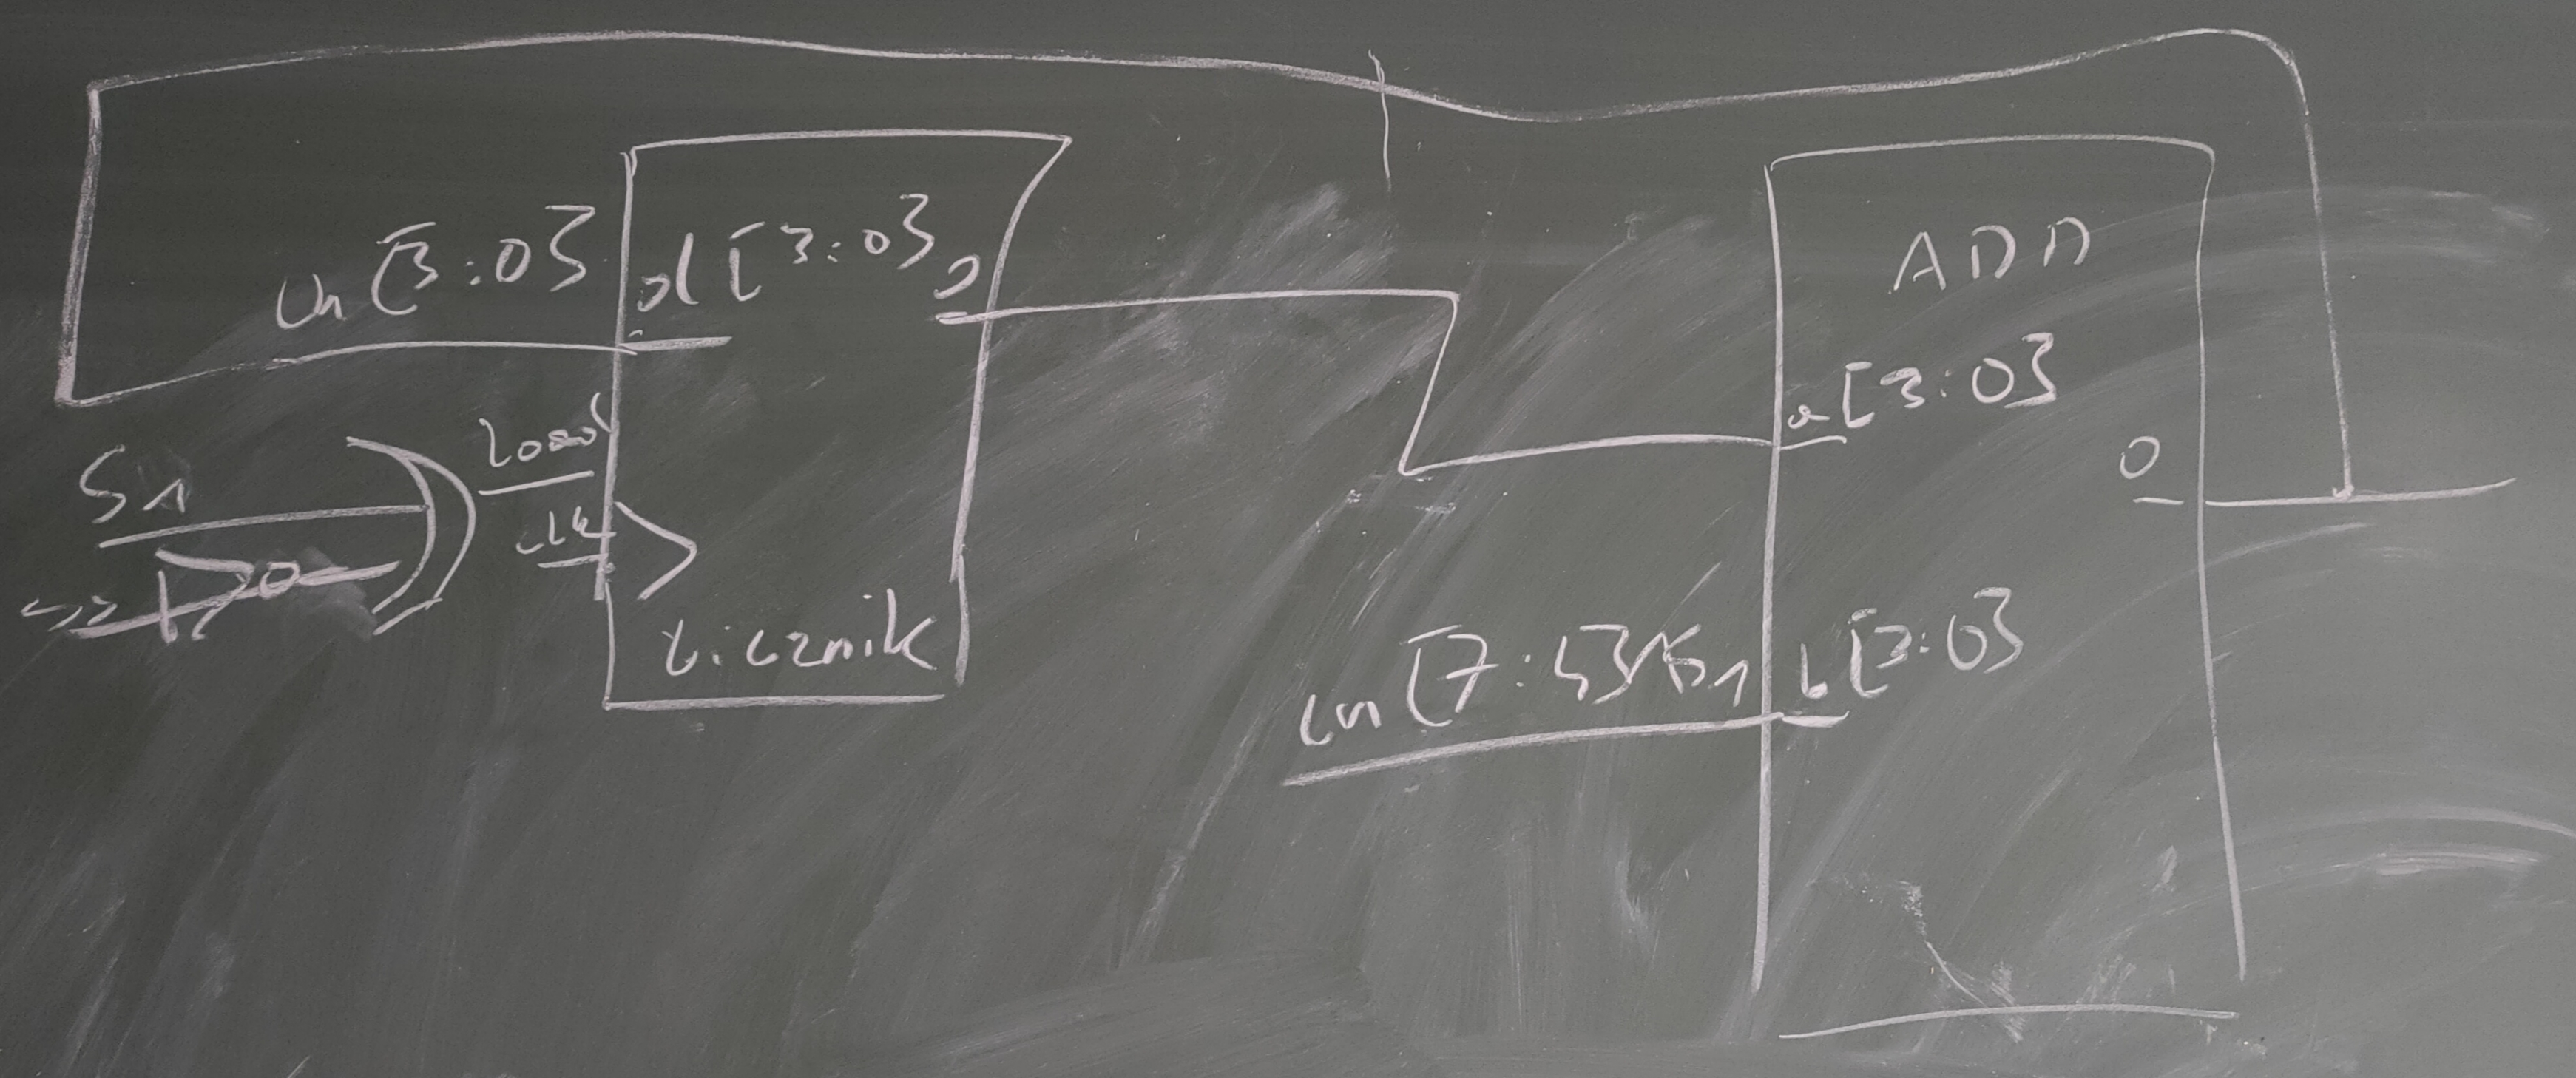
\includegraphics[scale=0.1]{./L08Z03.jpg}
\end{center}
\section{Jaka będzie wartość e po jednym cyklu zegara, jeśli wartość ra i rb przed tym cyklem była równa 1, dla poniższych bloków? Dlaczego?}
\begin{center}
	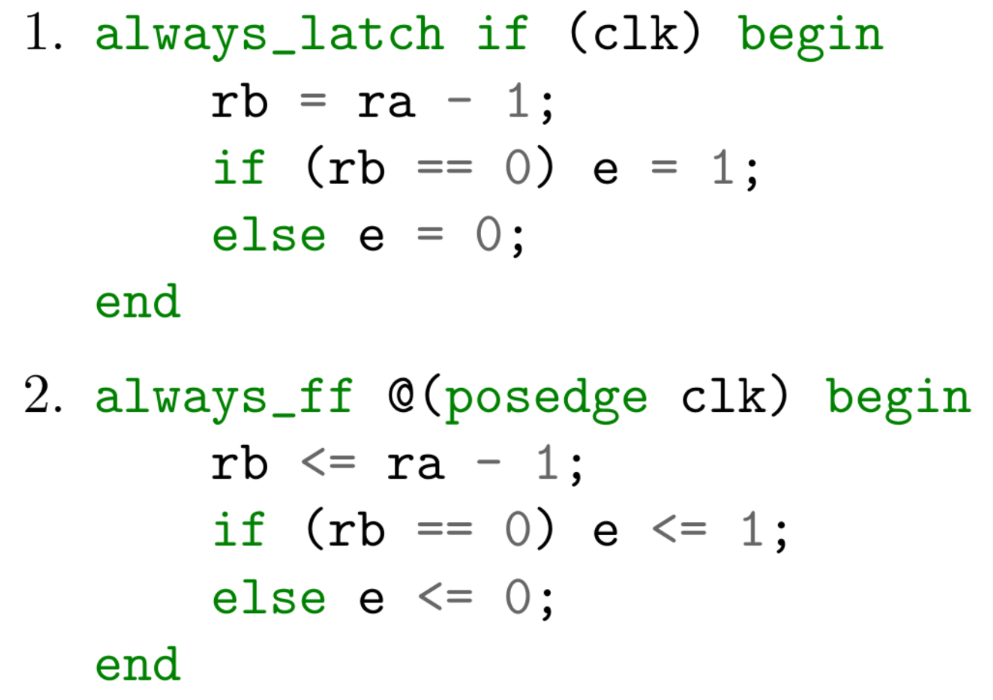
\includegraphics[scale=0.4]{./L08Z04.png}\\
\end{center}
Oturz dla pierwszego $e=1$, natomiast dla drugiego $e=0$, jest tak ponieważ operator $=$ przypisuje od razu, $<=$ natomiast odracza aby operacje były współbieżne.
\section{(2 pkt) Zaimplementuj przy użyciu układu sekwencyjnego algorytm Euklidesa (w wariancie z odejmowaniem) znajdujący największy wspólny dzielnik (NWD) dwóch liczb 16-bitowych bez znaku. Podążaj przy tym za metodą przedstawioną na wykładzie na przykładzie obliczania silni. W szczególności, proszę podać:}
\begin{itemize}
\item potrzebne sygnały wejściowe i wyjściowe oraz ich rozmiar,
\item potrzebne rejestry oraz ich rozmiar, należy postarać się nie wprowadzać zbędnego stanu,
\item zależność stanu w następnej chwili czasu od stanu w poprzedniej chwili czasu oraz wejść,
\item schemat układu, bez rozpisywania poszczególnych bramek,
\item implementację w SystemVerilogu.
\end{itemize}
\begin{lstlisting}[language=Verilog] 
module GCD(input clk,
           input [15:0] a,
           input [15:0] b,
           input ini,
           output [15:0]e,
           output fin
          	);
  assign fin = (!newb || !newa);
  logic [15:0]newa;
  logic [15:0]newb;
  assign e = fin ? (newb==0 ? newa : newb) : 0;
  always_ff @(posedge clk)
    if(ini) begin
      newa <= a;
      newb <= b;
    end else if(newa > newb) begin
	  newa <= newa-newb;
  	  newb <= newb;
    end else begin
      newa <= newa;
      newb <= newb-newa;
    end  
endmodule
\end{lstlisting}

\end{document}